%%%%%% 第2章 %%%%%%%%%%%%%%%%%%%%%%%%%%%
%
%\chapter{マッチング処理制約を伴う4工程FFS} \label{sec:chapter2}
%
%\chaptermark{4工程FFS}
%
%\section{4工程FFS\label{sec:zhangffs}}
%文献$\cite{siryo1}$で考察されたマッチング処理制約のある4工程FFSを考える.
%図$\ref{fig:ffs}$に4工程FFSにおける各工程の作業と工程間の関係を図示する.
%第1工程では二種類の部品がそれぞれ別々に到着し,その部品を独立のラインで加工し第2工程へ渡す.
%第2工程はマッチング工程と呼ばれ,二つの部品を1度組み合わせて加工し,その後再び二つの部品に分解して次の第3工程へ渡す.
%このとき第2工程で1度組み合わされた二つの部品はペアとなる.
%第3工程では第2工程で分解した二つの部品をそれぞれ別のラインで並列的に加工する.
%最後の第4工程は組み合わせ工程と呼ばれ,二つの部品を組み合わせてシステムから離脱させる.
%このとき第4工程で組み合わされる二つの部品は第2工程で処理されたペアでならなければならないという制約があり,これをマッチング処理制約と呼ぶ.
%また,各工程には部品を配置するバッファが用意されており,次工程のバッファが埋まっている場合,前工程から部品を渡すことができないため前工程の処理が止まる.
%これをブロッキングと呼ぶ.
%図$\ref{fig:ffs}$のFFSにおいて,部品の追い抜きがなく,部品の順序が保持される場合,第4工程における各バッファの先頭の二つの部品は必ず第2工程で処理されたペアであるためマッチング処理制約が満たされる.
%
%
%
%\begin{figure}[t]
%	\begin{center}
%		\includegraphics[width=\hsize]{model_ver5.eps}
%	\end{center}
%	\caption{マッチング工程のある4工程FFS.}
%	\label{fig:ffs}
%\end{figure}
%
%
%\begin{figure}[h]
%	\begin{center}
%		\includegraphics[clip, width=\hsize]{queue-ori.eps}
%	\end{center}
%	\caption{4工程FFSに対する待ち行列ネットワークモデル.}
%	\label{fig:queue}
%\end{figure}
%
%文献$\cite{siryo1}$では上述のFFSを,二種類の部品の第1工程への到着が到着率$\lambda$のポアソン過程,各工程での処理が平均$\frac{1}{\mu}$の指数分布に従う,待ち行列ネットワークモデルで表現した.
%図 \ref{fig:queue} はZhangら $\cite{siryo1}$ によるマッチング処理制約のある4工程FFSに対する待ち行列ネットワークモデルを表している.
%ここで,白丸は部品を処理する機械,白丸についている長方形は各機械のバッファを表現し,各矢印は機械によって処理された部品の移動を表しており,バッファを指していればそのバッファへ,何もない場所を指している場合システムからの離脱を意味する.
%
%\clearpage
%
%
%
%\section{解析手法}
%本論文では,4工程FFSの待ち行列ネットワークモデルを一般化確率ペトリネット(GSPN)で書き換える.
%その後,GSPN解析ツールを通じて連続時間マルコフ連鎖へ変換した後に,連続時間マルコフ連鎖の定常解析を行う.
%これにより解析的に厳密な性能評価指標が導出できる.
%図 \ref{fig:original}は図\ref{fig:queue}の待ち行列ネットワークをGSPNに書き換えたものである.
%GSPNの詳細については付録 \ref{sec:app}を参照されたい.
%
%
%
%\begin{figure}[h]
%	\begin{center}
%		\includegraphics[height=0.6\vsize]{original.eps}
%	\end{center}
%	\caption{4工程FFSの待ち行列ネットワークに対応するGSPN.}
%	\label{fig:original}
%\end{figure}
%

\chapter{4 step FFS with match processing constraint} \label{sec:chapter2}

\chaptermark{4 step FFS}

\section{4 step FFS \label{sec:zhangffs}}
We think about 4 step FFS with match processing constraint considered in bibitem $\cite{siryo1}$.
Figure $\ref{fig:ffs}$ shows the processs in each step and relationship between steps in 4 step FFS.
In the first step,  two types of parts arrive separately and the parts are processed on independent lines and handed to the next step.
The second step is called a matching step and in this step, two parts are combined once and processed. After processed, two parts are disassembled and then passed to next step.
Here, the two parts combined once in step 2 will be pairs.
In the third step, the two parts decomposed in the second step are processed in parallel on separate lines.
The final fourth step is called combine step. The two parts are combined in this step and shipped from system.
At this time, there are constraint that two parts combined at the fourth step must be pairs processed in the second step, and this constraint is called match processing constraint.
Also, in each step, a buffer for parts is prepared, and when the buffer of the next step is full, processing of the previous step would stop since parts can not be tranferred from the previous step.
This is called blocking.
For the FFS illustrated in figure $\ref{fig:ffs}$, if there is no overtaking of parts and the order of parts is maintained, the two parts at the head of each buffer in the fourth step are always pairs processed in the second step, so the match processing constraint is satisfied.

\begin{figure}[t]
	\begin{center}
		\includegraphics[width=\hsize]{fig/model_ver5.eps}
	\end{center}
	\caption{4 step FFS with match processing constraint.}
	\label{fig:ffs}
\end{figure}


\begin{figure}[h]
	\begin{center}
		\includegraphics[clip, width=\hsize]{fig/queue-ori-eng.eps}
	\end{center}
	\caption{Queuing network model for 4 step FFS.}
	\label{fig:queue}
\end{figure}

Zhang et al. $\cite{siryo1}$, represented the FFS above with the queueing network with arrival of the two kinds of parts to the first step follows the Poisson process of the arrival rate $\lambda$, and the processing at each step follows the exponential distribution with the average $\frac{1}{\mu}$.
Figure \ref{fig:queue} shows 4 step FFS with match processing constraint used by Zhang et al.
In this figure, white circle represent the machines for processing parts, rectangles on white circles represent buffers of each machine, each arraow represents movement of parts processed by the machine.
If the arrow points to an empty place,, it means departing from the sysytem.

\clearpage


\section{Analystic method}
In this paper, we rewrite queuing network model of 4 step FFS with Generalized Stochastic Petri Net (GSPN).
After that, we convert GSPN to continuous-time Markov chain (CTMC) throught GSPN analysis tool, and do steady state analysis of CTMC for performance evaluation.
Analytically strict performance evaluation can be derived by this method.
FIgure \ref{fig:original} shows GSPN which rewritten queuing network of figure \ref{fig:queue} .
For details of GSPN, see appendix \ref{sec:app}.

\begin{figure}[h]
	\begin{center}
		\includegraphics[height=0.6\vsize]{fig/original.eps}
	\end{center}
	\caption{GSPN correspond for queuing network of 4 step FFS.}
	\label{fig:original}
\end{figure}


